\chapter{Preliminary  Design}

\section{Tools of data flow strategy}
	Data flow strategy shows th and their interactions...........\\
\textbf{Data flow analysis makes use of the following tools:}\\
Flow Charts\\
Data Flow Diagrams\\
Data Dictionary\\
\textbf{Flowchart}\\
Flowchart is used to represent the algorithm .......\\
\textbf{Data Dictionary}\\
The logical characteristics of current systems data stores, including name, description, aliases, contents, ..........\\
\textbf{Data Structure Diagrams}\\
A pictorial description of the relation between entities (people, places, events and things) in system and the set of information about the entity, .........\\
\textbf{Structured Chart}\\
A design tool that pictorially shows the relation between processing modules in computer software, describes .............


%-----------------------------------------------------------------

\section{Use Case Diagram}
%If you add information about use case diagram\\
\subsubsection{Usecase Diagram For Admin}
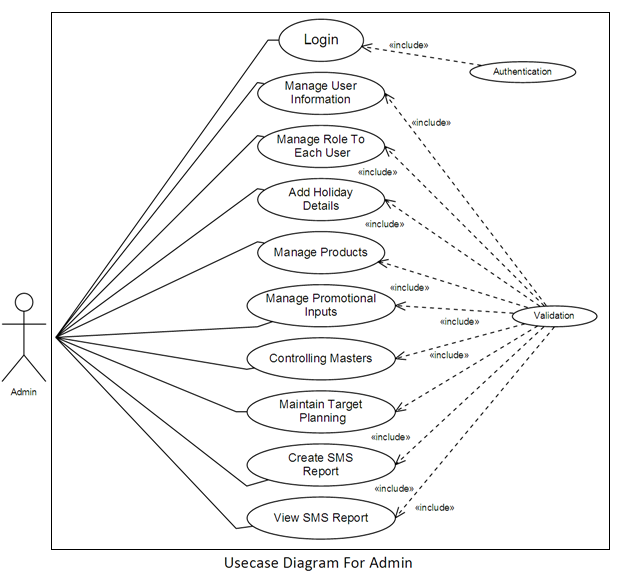
\includegraphics[scale=0.7]{Diag/usecaseadmin.png}

\label{fig:Use case diagram For Admin}
\subsubsection{Usecase Diagram For Other Users.}
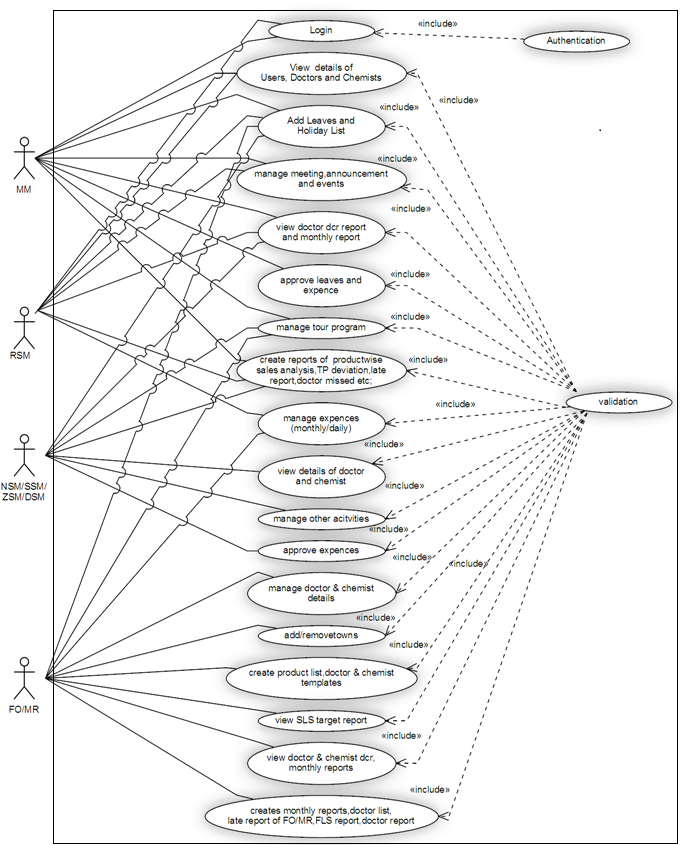
\includegraphics[scale=0.8]{Diag/usecaseall.png}

\label{fig:Use case diagram For Other User}



%-----------------------------------------------------------------
%\section{Activity Diagram}
%%If you add information about Activity Diagram\\
%
%\includegraphics[scale=.8]{Diag/activitylogin.png}
%\label{fig:Activity Diagram}



%-----------------------------------------------------------------

\section{Entity Relationship Diagram}

\subsubsection{ERD For Chemist.}
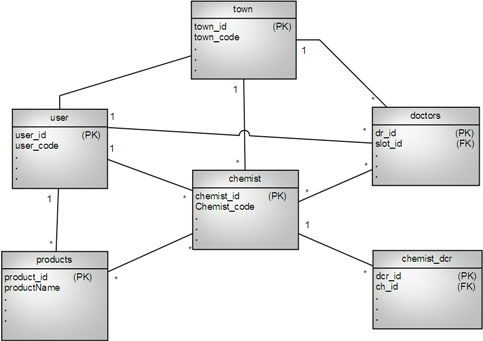
\includegraphics[scale=0.7]{Diag/ERDchemist.png}
\label{abc}

\subsubsection{ERD For doctor.}
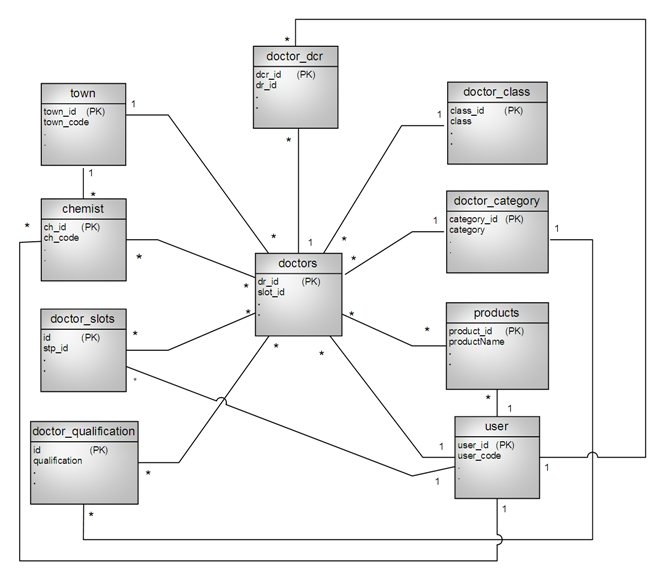
\includegraphics[scale=0.7]{Diag/ERDdoctor.png}
\label{abc}


%\subsubsection{ERD For users.}
%\includegraphics[scale=0.7]{Diag/ERDuser.png}
%\label{abc}
%
%\subsubsection{ERD For Products.}
%\includegraphics[scale=0.7]{Diag/ERDprod.png}
%\label{abc}
%-----------------------------------------------------------------

\section{Data Flow Diagram}
%If you add information about Data flow diagram\\

%\begin{figure} [h]
%\begin{center} 
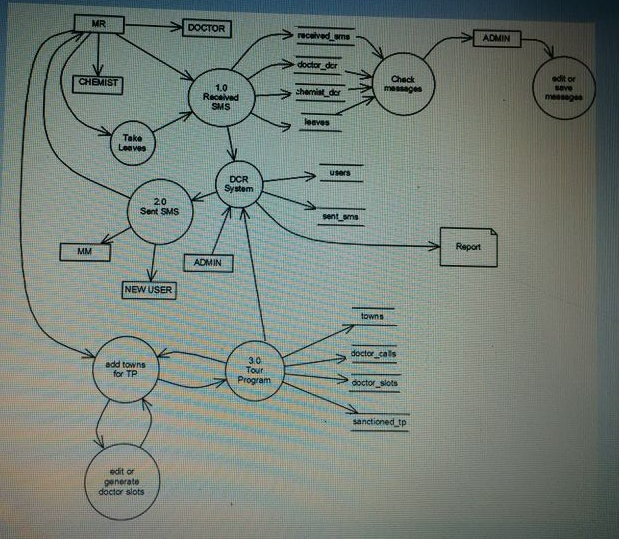
\includegraphics[scale=.9]{Diag/d1.png}
\label{fig:Contex Level}
%\end{center}
%\end{figure}



%\begin{figure} [h]
%\begin{center} 
%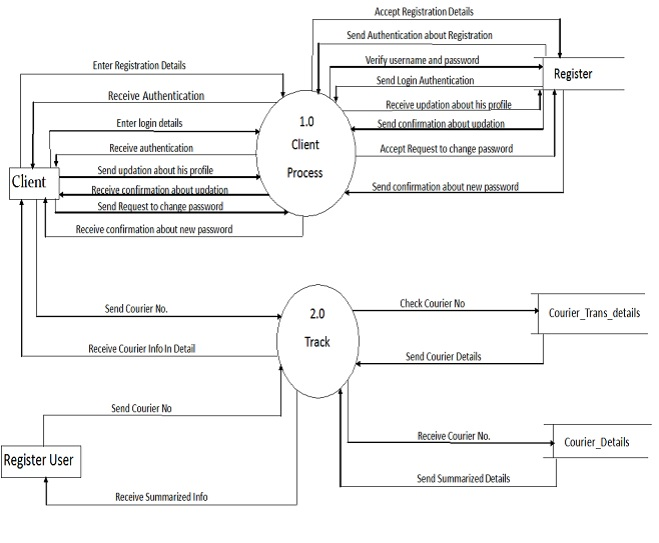
\includegraphics[scale=.9]{Ch5/dfd2.jpg}
%Fig. Data Flow Diagram
%\label{fig:DFD2}


\